The general equation of a circle is 
\begin{align}
\label{sep/2/6/eq:1}
\Vec{x}\Vec{x}^\top - 2 \Vec{O}^\top \Vec{x} + \norm{O}^{2}-r^2=0
\end{align}
Given equation of the circle is
\begin{align}
\label{sep/2/6/eq:2}
\Vec{x}\Vec{x}^\top = 4
\end{align}
Comparing \eqref{sep/2/6/eq:2} with \eqref{sep/2/6/eq:1}, we get
\begin{align}
\label{sep/2/6/eq:3}
\Vec{O}=\myvec{0 \\ 0}\\
\label{sep/2/6/eq:4}
r=2
\end{align}
Given lines are
\begin{align}
\label{sep/2/6/eq:5}
L_{1}: \: \Vec{x}=\myvec{0 \\ 0} + \alpha \myvec{0 \\ 1} \\
\label{sep/2/6/eq:6}
L_{2}: \: \Vec{x}=\myvec{2 \\ 0} + \beta \myvec{0 \\ 1}
\end{align}
where $\alpha$ and $\beta$ are real numbers.
We know the points of intersection of the line
\begin{align}
\label{sep/2/6/eq:7}
L: \: \Vec{x}=\Vec{q}+\mu\Vec{m}
\end{align}
with the circle in \eqref{sep/2/6/eq:2} is given by 
\begin{align}
\label{sep/2/6/eq:8}
\Vec{x_{i}}=\Vec{q}+\mu_{i}\Vec{m}
\end{align}
where 
\begin{multline}
\mu_{i} = \frac{1}{\Vec{m}^\top \Vec{I}\Vec{m}}\lbrak{-\Vec{m}^\top\brak{\Vec{I}\Vec{q}+\Vec{O}}}\\
\rbrak{\pm \sqrt{\sbrak{-\Vec{m}^\top\brak{\Vec{I}\Vec{q}+\Vec{O}}}^2-\brak{\Vec{q}^\top\Vec{I}\Vec{q}+\Vec{O}^\top\Vec{q}-r^2}\brak{\Vec{m}^\top \Vec{I}\Vec{m}}}}
\end{multline}
Solving for $\alpha$ and $\beta$, we get
\begin{align}
\label{sep/2/6/eq:10}
\alpha&=\pm 2 & \beta&=0
\end{align}
Points of intersection of line $L_{1}$ are $\myvec{0\\2}$ and $\myvec{0 \\ -2}$ and line $L_{2}$ is $\myvec{0 \\ 0}$.\\
The angle made by lines $L_{1}$ and $L_{2}$ with the x axis i.e $\myvec{0 & 1}\Vec{x}=0$ is
\begin{align}
%\label{sep/2/6/eq:10}
\cos \theta = {}&\frac{\myvec{1 \\ 0}^\top \myvec{0 & 1}}{\norm{\myvec{1 & 0}}\norm{\myvec{0 & 1}}}\\
\label{sep/2/6/eq:11}
={}& 0\\
\label{sep/2/6/eq:12}
\implies \theta = 90^{\circ}
\end{align}
The area of sector thus obtained is
\begin{align}
\label{sep/2/6/eq;13}
\frac{\theta^{\circ}}{360^{\circ}}\pi r^2 ={}&\frac{90^{\circ}}{360^{\circ}}\pi r^2\\
\label{sep/2/6/eq:14}
={}&\frac{\pi}{4}2^2\\
\label{sep/2/6/eq:15}
={}&\pi
\end{align}
\begin{figure}[!ht]
\centering
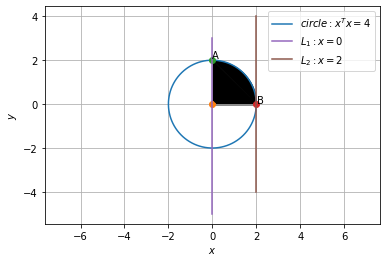
\includegraphics[width=\columnwidth]{solutions/sep/2/6/Figures/q5}
\caption{Plotting the region bounded by circle and lines in first quadrant}
\label{sep/2/6/fig}
\end{figure}

		

